%\documentclass[12pt,convert={density=150}]{standalone}
\documentclass[12pt]{standalone}

\usepackage{fontspec}
\usepackage{amsmath}
\usepackage{amsfonts}
\usepackage{amssymb}
\usepackage{tikz}

\usetikzlibrary{arrows}
\usetikzlibrary{intersections}

\begin{document}
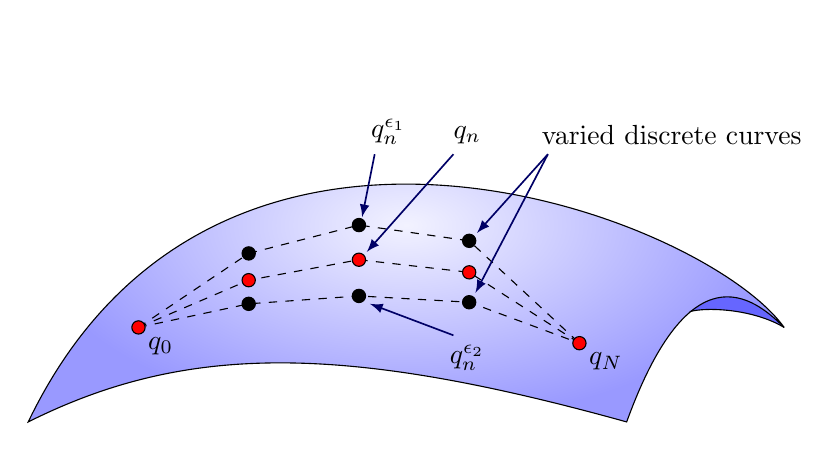
\begin{tikzpicture}[scale=2]%

\begin{scope}[fill = blue!60!white]
\clip (4.2, 0.0) rectangle (4.8,1.0);
\fill
   (3.8, 0.0) .. controls (4.2, 1.1) and (4.6, 0.8)  .. (4.8, 0.6)
-- (4.8, 0.6) .. controls (4.6, 0.72) and (4.3, 0.73) .. (4.2, 0.7);
\end{scope}

\draw [shading=axis, outer color=blue!40!white, inner color=blue!05!white]
   (4.8, 0.6) .. controls (4.3, 1.3) and  (1.2, 2.5) .. (0.0, 0.0)
-- (0.0, 0.0) .. controls (1.0, 0.5) and (2.0, 0.5)  .. (3.8, 0.0)
-- (3.8, 0.0) .. controls (4.2, 1.1) and (4.6, 0.8)  .. (4.8, 0.6);

\draw [name path=out4] (4.2, 0.7) .. controls (4.3, 0.73) and (4.6, 0.72) .. (4.8, 0.6);


%\draw [black, name path=curve1] (0.7, 0.6) .. controls (1.7, 1.5) and (2.9, 1.5) .. (3.5, 0.5);
%\draw [red,   name path=curve2] (0.7, 0.6) .. controls (1.7, 1.2) and (2.9, 1.2) .. (3.5, 0.5);
%\draw [black, name path=curve3] (0.7, 0.6) .. controls (1.7, 0.9) and (2.9, 0.9) .. (3.5, 0.5);

%\draw [latex-] (2.30, 1.25) .. controls (2.26, 1.18) and (2.24, 1.15) .. (2.233,1.06);
%\draw [latex-] (2.22, 0.82) .. controls (2.22, 0.90) and (2.22, 0.95) .. (2.229,1.01);


\draw [dashed] (0.7, 0.6) -- (1.4, 0.75) -- (2.1, 0.80) -- (2.8, 0.76) -- (3.5, 0.5);
\draw [dashed] (0.7, 0.6) -- (1.4, 0.90) -- (2.1, 1.03) -- (2.8, 0.95) -- (3.5, 0.5);
\draw [dashed] (0.7, 0.6) -- (1.4, 1.07) -- (2.1, 1.25) -- (2.8, 1.15) -- (3.5, 0.5);


\filldraw [black, fill=black] (1.4, 0.75) circle (1.2pt)
                              (2.1, 0.80) circle (1.2pt)
                              (2.8, 0.76) circle (1.2pt);

\filldraw [black, fill=red]   (1.4, 0.90) circle (1.2pt)
                              (2.1, 1.03) circle (1.2pt)
                              (2.8, 0.95) circle (1.2pt);

\filldraw [black, fill=black] (1.4, 1.07) circle (1.2pt)
                              (2.1, 1.25) circle (1.2pt)
                              (2.8, 1.15) circle (1.2pt);

\filldraw [black, fill=red] (0.7, 0.6) circle (1.2pt) node[black, anchor=north west] {$q_0$}
                            (3.5, 0.5) circle (1.2pt) node[black, anchor=north west] {$q_N$};


\draw [to-, line width=.6pt, blue!40!black, latex-] (2.15, 1.08) -- (2.7, 1.7) node[black, anchor=south] {$\quad q_{n}$};
\draw [to-, line width=.6pt, blue!40!black, latex-] (2.12, 1.30) -- (2.2, 1.7) node[black, anchor=south] {$\quad q_{n}^{\epsilon_{1}}$};
\draw [to-, line width=.6pt, blue!40!black, latex-] (2.17, 0.75) -- (2.7, 0.55) node[black, anchor=north] {$\quad q_{n}^{\epsilon_{2}}$};

\draw [to-, line width=.6pt, blue!40!black, latex-] (2.85, 1.20) -- (3.3, 1.7);
\draw [to-, line width=.6pt, blue!40!black, latex-] (2.84, 0.82) -- (3.3, 1.7);
\draw (3.2, 1.7) node[black, anchor=south west] {varied discrete curves};



%\draw [line width=0pt, name path=int1] (1,0) -- (1,2);

%\fill [name intersections={of=curve1 and int1, by={a}}]
%        (a) circle (2pt);

\end{tikzpicture}
\end{document}
